\documentclass{llncs}

\usepackage{graphicx}

\begin{document}

\title{Artificial Neural Networks Time Series Forecasting with Android Live Wallpaper Technology} 

\author{Petar Tomov, Iliyan Zankinski, Maria Barova}

\institute{Institute of Information and Communication Technologies \\
Bulgarian Academy of Sciences \\
acad. Georgi Bonchev Str, block 2, office 514, 1113 Sofia, Bulgaria \\
\email{p.tomov@iit.bas.bg} \\
\texttt{http://www.iict.bas.bg/}}

%----------------------------------------------------------------------------------------
%   Title
%----------------------------------------------------------------------------------------

\maketitle

%----------------------------------------------------------------------------------------
%   Abstract
%----------------------------------------------------------------------------------------

\begin{abstract}
The application of Artificial Neural Networks (ANN) for time series forecasting is quite common in the last few decades \cite{atanasova01}. ANN may be adopted in a variety of topologies and training algorithms. Algorithms can be sequential, but they can also be performed in parallel. Computing device types used for training ANN may vary from supercomputers, grid networks and single desktop computers to mobile devices. The focus of this research is training of ANN for Time Series Forecasting (TSF) as background calculations of Android Live Wallpaper technology. 

\keywords{artificial neural networks, mobile computing, time series forecasting}
\end{abstract}

%----------------------------------------------------------------------------------------
%   Paper
%----------------------------------------------------------------------------------------

\section{Introduction}

In their nature, common types of ANNs are weighted directed graphs \cite{balabanov03}. The process of ANN training aims to find such values for the weights which minimize the total error of the output \cite{balabanov04}. When the size of ANN is larger, the amount of weights may reach very high levels. With the increase of the number of weights, the velocity of training of a single ANN on a single computer is being reduced. The elevated amount of calculations poses the application of supercomputers, clusters, GRIDs and donated distributed computing networks as reasonable and adequate \cite{balabanov01,balabanov02,keremedchiev01,tomov01}. In the last decade the immense spread of mobile devices suggests their surpassing usage over stand alone computers. During most of the operating time, the mobile devices are in idle mode. The possibilities ANN to be trained in distributed computing environment and the use of mobile devices can be efficiently combined in software system for ANN training on mobile operating systems such as Android. In the current research Android Live Wallpaper technology is involved in ANN training for time series forecasting.

\section{Technical Solution}

The technical solution is divided in two parts. The first one is related to the Android application itself. The second one is related to the ANN data structure representation, information representation and the process of training/forecasting. For the first part Android development capabilities are used while for the second part Ecoge programming library is involved. 

\subsection{Android Live Wallpaper}

Live Wallpaper is interactive background on the Android home screen, which can even process animation. The Live Wallpaper does not differ much from other Android applications. First step of Live Wallpaper creation is an XML file with application description (manifest). Second component is a Service class inherited from WallpaperService. Inside of the Service class there is an Engine class. The Engine object is responsible for training/forecasting execution and background redrawing. Running LW on the Android operating system requires special permissions. The use of Live Wallpaper feature should be explicitly written into the manifest file in order to prevent wallpaper installation on devices which are not capable of running it. 

\begin{figure}[h]
  \centering
  \includegraphics[width=0.5\linewidth]{fig01}
  \caption{Android Live Wallpaper settings screen.}
\label{fig:01}
\end{figure}

The set up the wallpaper is performed by sending an Intent to the operating system. SQLite database is used to store financial time series in the mobile device for offline mode operation. On regular intervals, wallpaper service is activated - cycle of training is executed, forecast is retrieved and the visual information is updated. Settings screen is used for visual representation parameters and device loading options (Fig. \ref{fig:01}). During operating mode a background image is drawn and ANN training/forecasting information is displayed (Fig. \ref{fig:02}). 

\begin{figure}[h]
  \centering
  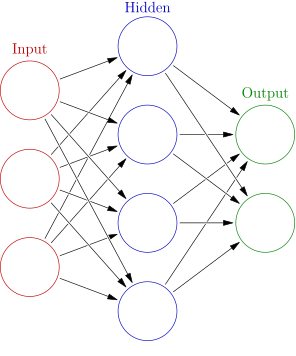
\includegraphics[width=0.5\linewidth]{fig02}
  \caption{Android Live Wallpaper operational screen.}
\label{fig:02}
\end{figure}

\subsection{Encog Machine Learning Framework}

For the process of forecasting, Econg library is used. Multilayer perceptron with 3 layers is chosen. Time series is conditionally divided in two parts (past and future). Data frame for the past (lag) is supplied at the input of the ANN. Data frame for the the future (lead) is expected at the output of the ANN. Time series data are scaled (according neurons activation function) before fed into ANN's input. The output is also scaled with the opposite scaling coefficient used at the input. At each training cycle resilient backpropagation training is executed. 

\section{Conclusions}

As per the results of the current research, the application of donated mobile devices power appears to be much more promising even compared to the donated desktop distributed computing, given that mobile devices are almost always running, which is not the case with the desktop computers. As future studies, donated mobile distributed computing infrastructure can be efficiently used for experiments with different activation functions \cite{zankinski01} or permutation algorithms \cite{zankinski02}. Other interesting research areas where mobile distributed computing can be applied are barcode readers \cite{atanasova02} and computer networks traffic analysis \cite{tashev01,tashev02}.

%----------------------------------------------------------------------------------------
%   Acknowledgements
%----------------------------------------------------------------------------------------

\section*{Acknowledgements}

This work was supported by private funding of Velbazhd Software LLC.

%----------------------------------------------------------------------------------------
%   Bibliography
%----------------------------------------------------------------------------------------

\begin{thebibliography}{99}

\bibitem{atanasova01} Atanasova, T., Barova, M., Balabanov, T., \textit{Use of Neural Models for Analysis of Time Series in Big Data}, Publishing complex of "Vasil Levski" National Military University, ISSN 1314-1937, 193--198, 2016.

\bibitem{atanasova02} Atanasova, T., Atanasov, J., \textit{Business Processes Traceability in SME by Barcode System}, Proceedings of the International Scientific Conference, UNITECH’16, Gabrovo, Bulgaria, ISSN 1313-230X,  207--212, 2016.

\bibitem{balabanov01} Balabanov, T., Genova, K., \textit{Distributed System for Artificial Neural Networks Training Based on Mobile Devices}, Proceedings of the International Conference Automatics and Informatics, Sofia, Bulgaria, Federation of the Scientific Engineering Unions John Atanasoff Society of Automatics and Informatics, ISSN 1313-1850, 49--52, 2016.

\bibitem{balabanov02} Balabanov, T., Keremedchiev, D., Goranov, I., \textit{Web Distributed Computing For Evolutionary Training Of Artificial Neural Networks}, International Conference InfoTech, Varna - St. St. Constantine and Elena resort, Bulgaria, Publishing House of Technical University - Sofia, ISSN 1314-1023, 210--216, 2016.

\bibitem{balabanov03} Balabanov, T., Zankinski, I., Barova, M., \textit{Strategy for Individuals Distribution by Incident Nodes Participation in Star Topology of Distributed Evolutionary Algorithms}, Cybernetics and Information Technologies, Institute of Information and Communication Technologies - BAS, vol. 16, no. 1, ISSN 1311-9702, 80--88, 2016.

\bibitem{balabanov04} Balabanov, T., Zankinski, I., Dobrinkova, N., \textit{Time Series Prediction by Artificial Neural Networks and Differential Evolution in Distributed Environment}. Proceedings of the International Conference on Large-Scale Scientific Computing, Sozopol, Bulgaria, Lecture Notes in Computer Science, Springer, vol. 7116, no. 1, ISBN 978-3-642-29842-4, 198–205, 2011. 

\bibitem{keremedchiev01} Keremedchiev, D., Barova, M., Tomov, P., \textit{Mobile Application as Distributed Computing System for Artificial Neural Networks Training Used in Perfect Information Games}, Proceedings of the International Scientific Conference, UNITECH’16, Gabrovo, Bulgaria, ISSN 1313-230X, 389--393, 2016.

\bibitem{tashev01} Tashev, T., Marinov, M., Monov, V., Tasheva, R., \textit{Modeling of the MiMa-algorithm for crossbar switch by means of Generalized Nets}, Proceedings of the 2016 IEEE 8th International Conference on Intelligent Systems (IS), Sofia, Bulgaria, ISBN 978-1-5090-1354-8, 593--598, 2016.

\bibitem{tashev02} Tashev, T., Monov, V., \textit{Modeling of the hotspot load traffic for crossbar switch node by means of generalized nets}, Proceedings of the 6-th International IEEE Conference Intelligent Systems IS'12, Sofia, Bulgaria, vol. 2, 187--191, 2012.

\bibitem{tomov01} Tomov, P., Monov, V., \textit{Artificial Neural Networks and Differential Evolution Used for Time Series Forecasting in Distributed Environment}, Proceedings of the International Conference Automatics and Informatics, Sofia, Bulgaria, ISSN 1313-1850, 129--132, 2016.

\bibitem{zankinski01} Zankinski, I., Tomov, P., Balabanov, T., \textit{Alternative Activation Function Derivative in Artificial Neural Networks}, 25th Symposium with International Participation - Control of Energy, Industrial and Ecological Systems, Bankya, Bulgaria, John Atanasoff Union of Automation and Informatics, ISSN 1313-2237, 79--81, 2017.

\bibitem{zankinski02} Zankinski, I., Stoilov, T., \textit{Effect of the Neuron Permutation Problem on Training Artificial Neural Networks with Genetic Algorithms in Distributed Computing}, Proceedings of the 24th International Symposium Management of Energy, Industrial and Environmental Systems, ISSN 1313-2237, Bankya, Bulgaria, 53--55, 2016.

\end{thebibliography}

\end{document}

